%-----------------------------------------------------------------------
% 
%-----------------------------------------------------------------------
%
%     
%
%
%%%%%%%%%%%%%%%%%%%%%%%%%%%%%%%%%%%%%%%%%%%%%%%%%%%%%%%%%%%%%%%%%%%%%%%%


\documentclass[twoside]{article}
\usepackage{amsmath,amsthm,amssymb,verbatim}

%     If your article includes graphics, uncomment this command.
\usepackage{graphicx}

%     If the article includes commutative diagrams, ...
%\usepackage[cmtip,all]{xy}

\usepackage{url}

\usepackage{fancyhdr}
\pagestyle{fancy}

\def\blfootnote{\xdef\@thefnmark{}\@footnotetext} 
\long\def\symbolfootnote[#1]#2{\begingroup%
\def\thefootnote{\fnsymbol{footnote}}\footnote[#1]{#2}\endgroup} 

	\addtolength{\oddsidemargin}{1cm}
	\addtolength{\evensidemargin}{-1cm}

\setcounter{page}{1}

\begin{document}

%     If you need symbols beyond the basic set, uncomment this command.
%\usepackage{amssymb}


\newtheorem{theorem}{Theorem}[section]
\newtheorem{lemma}[theorem]{Lemma}

\theoremstyle{definition}
\newtheorem{definition}[theorem]{Definition}
\newtheorem{example}[theorem]{Example}
\newtheorem{xca}[theorem]{Exercise}

\theoremstyle{remark}
\newtheorem{remark}[theorem]{Remark}

\numberwithin{equation}{section}


\date{}
\lhead[]{}
\chead[\underline{head}]{\it{O. Shanker}}
\rhead[]{}

% \title[short text for running head]{full title}
\title{\bf{Critical Behaviour for Riemann zeta? Sharp Transition}}

\maketitle


%    author one information
% \author[short version for running head]{name for top of paper}
\author{{\textbf{O. Shanker}},}
\thanks{ Mountain View, CA 94041, U. S. A. email: oshanker@gmail.com}

\thispagestyle{fancy}

%    Abstract is required.
\begin{abstract}
Abstract. 

\end{abstract}
{\textbf {Keywords}:} Critical behaviour, Riemann zeta,  
{\textbf {Mathematics Subject Classification (MSC)}:} 11M06, 11-04.


\symbolfootnote[0]{*}


\section{Introduction}

 There .


\section{\label{sec2}Materials and Methods}
Section Intro

\subsection{\label{seckaratsuba}xxx}

Among the many studies of large values of the Riemann zeta function on the critical axis, 
studied 
\begin{equation}
F(T; H)  \, = \, max_{|t-T| \le H} \zeta ( 0.5+it ) 
\label{eqRie}
\end{equation}
where $H$ is small compared to $T$. 

The freezing tra


\section{\label{conclusions}Conclusions}
We 

\begin{table}
\centering \(\begin{array}{cccccc}
\hline
Length~of  && Generalized &Gram&angle &\phi \\
Gram     &----&----&----&----&----\\
block  & -0.2\pi & -0.1\pi & 0.0\pi & 0.1\pi & 0.2\pi  \\
\hline
2 &3.167 &1.760 &1.000 &0.567 &0.316 \\
3 &7.323 &2.672 &0.993 &0.376 &0.138 \\
4 &20.958 &4.352 &0.982 &0.221 &0.043 \\
5 &170.829 &10.344 &1.041 &0.094 &0.008 \\
6 &1409.500 &35.516 &1.016 &0.023 &0.001 \\
\hline
\end{array}\)
\caption{Sharp transition in $Type~II/Type~I$ Gram block ratio at Gram point.
The statistics are from $1$ million Gram intervals at $t=10^{12}$.}
\label{tab:ratioE12}
\end{table}


\begin{figure*}
\centering
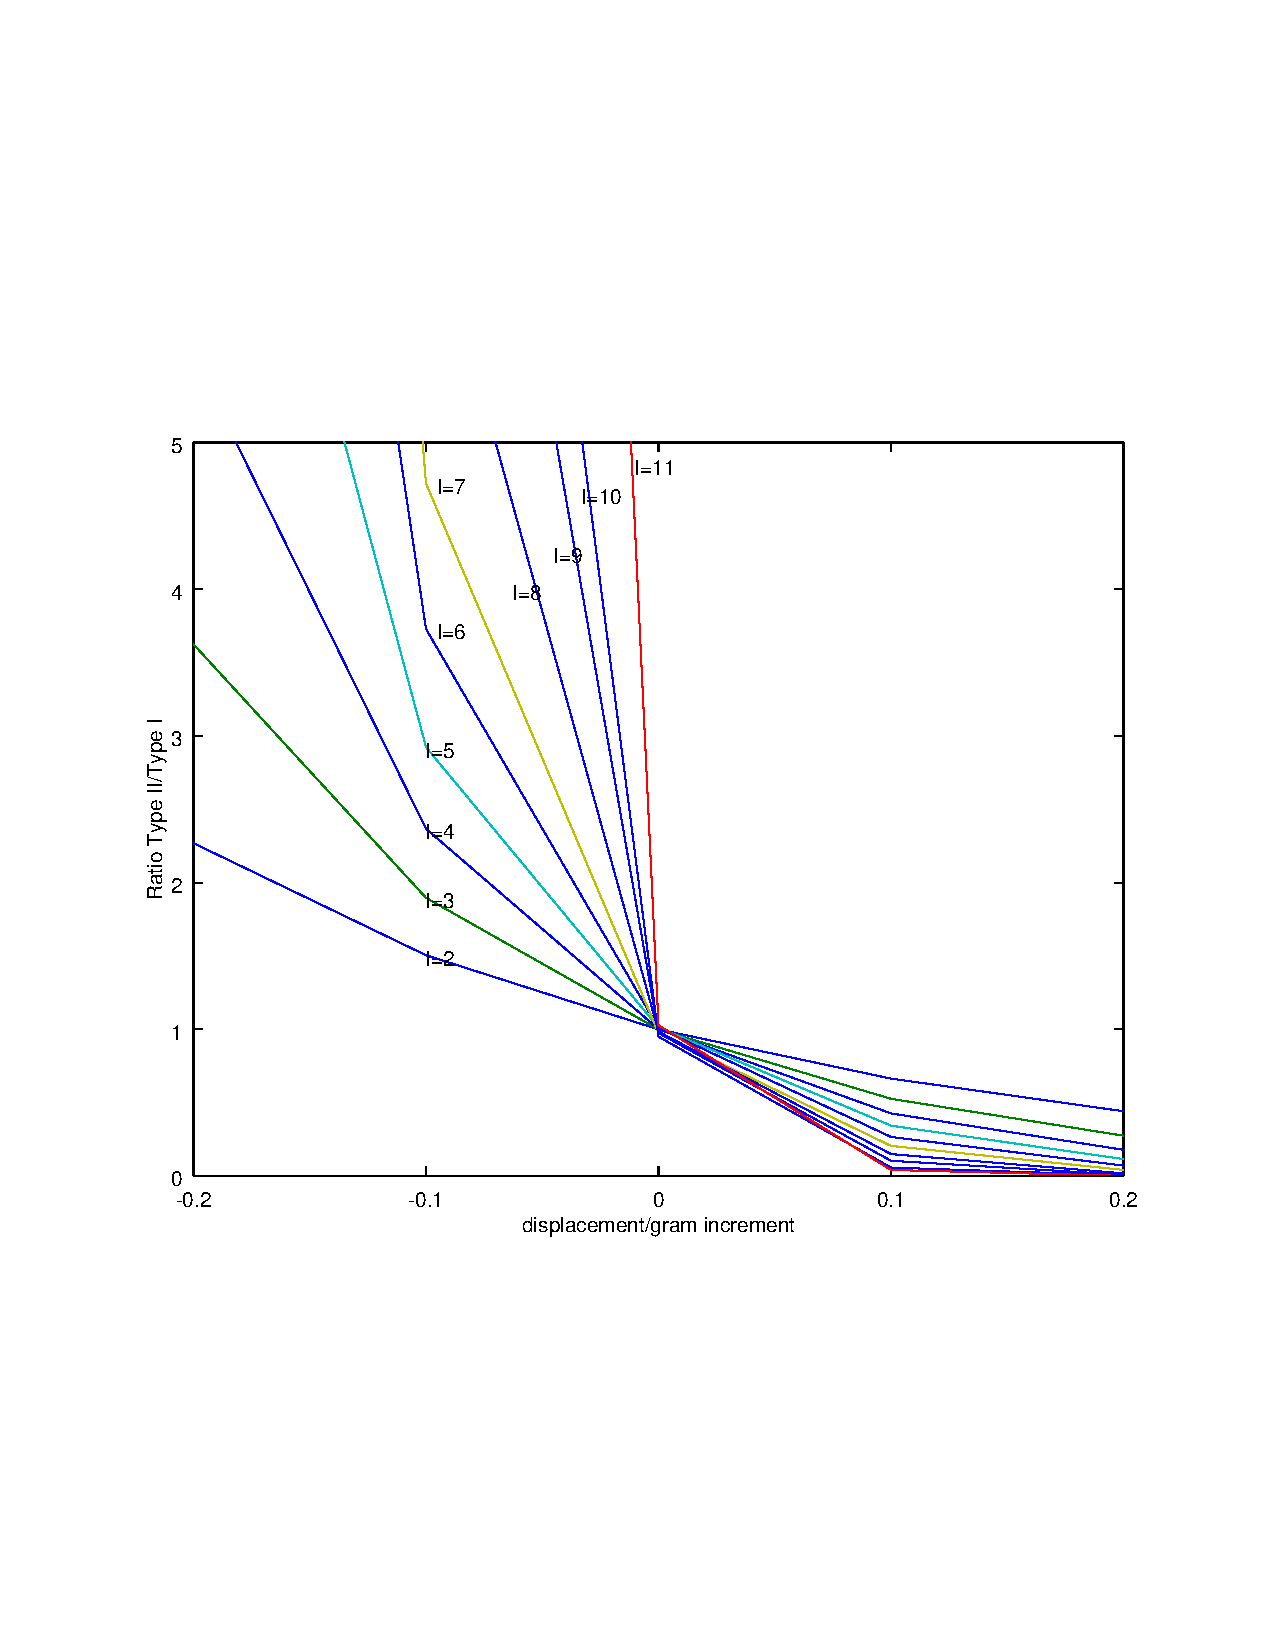
\includegraphics[width=1.0\textwidth]{typeIIratio.pdf}
\caption[]{ 
 Plot of  ratios in  Table~\ref{tab:ratioE28},  $t = 10^{28}$.
 }
\vspace{1mm}, 
\label{ratioE28}
\end{figure*}

\begin{table}
\centering \(\begin{array}{cccccc}
\hline
Length~of  && Generalized &Gram&angle &\phi \\
Gram     &----&----&----&----&----\\
block  & -0.2\pi & -0.1\pi & 0.0\pi & 0.1\pi & 0.2\pi  \\
\hline
2 &2.269 &1.505 &0.999 &0.664 &0.441 \\
3 &3.625 &1.896 &0.999 &0.526 &0.275 \\
4 &5.589 &2.367 &1.001 &0.427 &0.178 \\
5 &8.850 &2.923 &1.012 &0.343 &0.115 \\
6 &14.373 &3.729 &1.009 &0.266 &0.071 \\
7 &23.962 &4.722 &0.975 &0.205 &0.041 \\
8 &51.791 &6.715 &0.984 &0.149 &0.018 \\
9 &116.632 &10.130 &0.975 &0.104 &0.009 \\
10 &361.615 &13.306 &0.949 &0.058 &0.005 \\
11 &1397.000 &34.533 &1.028 &0.041 &0.001 \\
\hline
\end{array}\)
\caption{Sharp transition in $Type~II/Type~I$ Gram block ratio at Gram point.
The statistics are from $10$ million Gram intervals at $t=10^{28}$.}
\label{tab:ratioE28}
\end{table}


\section*{Acknowledgments and Funding Statement}

 The study was done as an independent researcher. There was no
external funding.

\section*{Ethical Compliance}

 No procedures were performed  involving human participants in the study.

\section*{Data Availability Statement}

The computer programs used during the current study are
available from the corresponding author on reasonable request.

\section*{Conflict of Interest declaration} 

The authors declare that they have no affiliations with or involvement in any organization 
or entity with any financial interest in the subject matter or materials discussed 
in this manuscript.


\bibliographystyle{amsplain}
\begin{thebibliography}{10}

\bibitem{osneural} O. Shanker, ``Neural Network prediction of Riemann zeta zeros''
{\it Advanced Modeling and Optimization}, {\bf 14}, 717-728, (2012), \url{tinyurl.com/4scve3nj}.


\bibitem{oscue} O. Shanker, 
``Random Matrix Theory explanation for Riemann Zeta Value Distribution Symmetry''
 report,
\url{https://tinyurl.com/ywhy4jsy}, 
(2022). 


\bibitem{Shanker 2018a} O. Shanker, 
``Good to Bad Gram Point Ratio For Riemann Zeta Function",
{\it Experimental Mathematics} {\bf 30}, 76-85,
\url{tinyurl.com/mwd5uwc5}(2021)

\bibitem{os6} O. Shanker, 
``Generalised Zeta Functions and Self-Similarity of Zero Distributions",
{\it J.  Phys. A} {\bf39}(2006), 13983-13997

\bibitem{Shanker 2018b} O. Shanker, 
``Symmetry properties of distribution of Riemann Zeta Function values on critical axis''
 report,
\url{tinyurl.com/47wj57b3}, 
(2018). 

\bibitem{Shanker 2020} O. Shanker, 
``Universality of Riemann Zeta Function value distribution on critical axis''
 report,
\url{tinyurl.com/yvbd2je6}, 
(2020). 




\end{thebibliography} 

\end{document}
